\documentclass[10pt]{extarticle} % article doctype, possible font size range from 8pt to 20pt with not all being avaiable.
\setcounter{secnumdepth}{4} % Max. section depth, e.g. 3 means 4.1.1 is possible but not 4.1.1.2
\title{\huge Technical Design Document MaramaUU Editor}
\author{Tim Hintzbergen, Wilbert Schepenaar, Thijs van Dam, Erik van Lune    \\s1097561, s1094484, s1078671, s1095043 (respectively)
\\\\ICTGPb
\\Wilco Moerman}
\date{May 15th, 2018}

% include packages
\usepackage{graphicx}
\usepackage{caption}
\usepackage{mathabx}
\usepackage{wrapfig}
\usepackage[margin=1.0in]{geometry} % Sets page margin, 2.0in is default.
\usepackage{titlesec}
\usepackage{hyperref}

% custom commands
\newcommand{\myparagraph}[1]{\paragraph{#1}\mbox{}\\} % Without \mbox{} all newlines will be ignored, making the first sentence appear on the same line as a paragraph title.

\DeclareCaptionFormat{cancaption}{#1#2#3\par} % Normal format actually
\DeclareCaptionLabelFormat{cancaptionlabel}{#1}
\captionsetup[figure][number]{format=cancaption,labelformat=cancaptionlabel}
\graphicspath { {images/} }
\begin{document}
    \nocite{*}
    \maketitle
    \thispagestyle{empty}
    \newpage
    %------------------------------------------------------------------------------------------------------------------------------------------------------- Introduction
    \newpage
    \setcounter{page}{1}
    \section {Introduction}
    This document contains all technical aspects of the product regarding the Editor.
    It describes the requirements, the architecture, the design choices and the epics.
    The requirements talk about all functional and non-functional requirements of the product.
    The architecture explains the form of the product, offers a clear overview and talks about some minute details.
    The list of design choices illustrates and defend the various choices that have been made during the design and construction of the product.
    Finally the epics list all coherent components of the product and their submodules
    \newpage

    \tableofcontents{}
    \newpage

    %------------------------------------------------------------------------------------------------------------------------------------------------------- Requirements
    \section{Requirements}
    Functional and Non-functional requirements.
    \newpage

    %------------------------------------------------------------------------------------------------------------------------------------------------------- Architecture
    \section{Architecture}
    WIP
    \begin{itemize}
        \item Sequence diagrams to show interactions between objects, if the interaction is particularly complex or involves many objects.
        \item Deployment diagrams to show the hardware and middleware on which the different software components run.
        \item Database designs, such as ERD diagrams.
        \item Descriptions of custom protocols, data formats etc.
        \item Security measures and considerations.
        \item Algorithm designs.
    \end{itemize}

    \subsection[class_diagram]{Class diagram}


    \subsubsection{Maramafication Loader}
    Underneath, the class diagram of the maramafication loader is shown.

    \begin{figure}[htb]
        \centering
        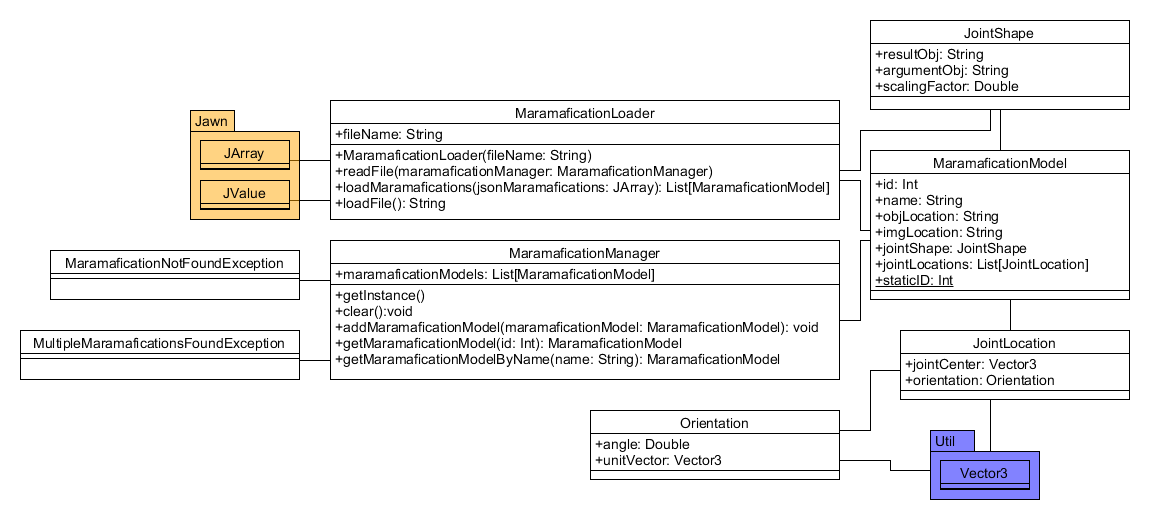
\includegraphics[width=\textwidth, height=\textheight, keepaspectratio]{Marama-Editor}
        \caption{Implementation of the maramafication loader and storing the maramafications}
    \end{figure}
    More information about the reasoning behind this particular structure is found inside the Design Choices\ref{sec:designchoices} section.
    In this section, the flow of the loader will be explained and how we end up with a list of MaramaficationModels.

    From the main thread, the MaramaficationLoader will be created, passing through the file (.mar) that has to be read.
    After that, the \textit{readFile()} method is called.
    This will respectively call the \textit{loadFile()} and the \textit{loadMaramafications()} methods.
    A string is constructed first, containing all the data of the file.
    Implying this file meets the standards, there will be a list of MaramaficationModels, with JointLocations and JointShapes inside of them in JSON format.
    Then, the Jawn library is used to parse the string. Due to the file being a list of MaramaficationModels, a JArray will be passed through the \textit{loadMaramafications()} method.
    \newpage
    \begin{figure}[htb]
        \center
        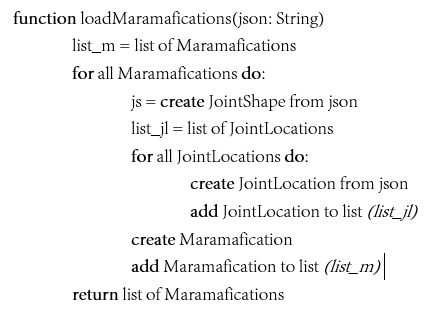
\includegraphics[width=60mm, keepaspectratio]{pseudocode}
        \caption{Pseudocode of the \textit{loadMaramafications()} method}
    \end{figure}

    The above pseudocode gives an idea of how the loadMaramafications method works.
    The list of Maramafications will finally be loaded inside the MaramaficationManager and the job is done.
    The MaramaficationManager being a singleton makes it accessible from the whole application, always being able to fetch the loaded MaramaficationModels.

    \subsection{Project Structure}
    Artifacts are built using sbt by passing the correct arguments, like so: \texttt{sbt assembly}.
    Sbt also manages the dependencies of the project.
    Next up is the documentation directory which, together with a local auxil directory make up our documentation, using \LaTeX\ of course.
    Finally there are a couple of build and property files together with the gitignore file.

    \newpage

    %------------------------------------------------------------------------------------------------------------------------------------------------------- Design Choices
    \section{Design Choices}\label{sec:designchoices}

    \subsection[Communication MVA-MEA]{Receiving command or information from MVA and MEA}
    \label{subsec:comchoice}
    In the ideal situation the Editor would be a command line tool for the Marama project.
    This way, it is easy to build a different, or more specialized view on top of the Editor.

    \subsection{Epics}
    \label{subsec:epics}
    The editor is made up of different epics.\\
    Epics are a collection of user stories that share a goal or functionality.

    \newcommand{\clickup}[1]{https://app.clickup.com/757520/761304/t/#1}

    \myparagraph{\href{\clickup{2e28f}}{\#2e28f} As a MD I want my maramafications to be added to the list inside the Marama-editor (loading .obj files)}



    \newpage

    %------------------------------------------------------------------------------------------------------------------------------------------------------- Build Automation
    \section{Continous Intergration}
    In this section build automation and its constituent components will be discussed.
    How we applied it, the software used and the targets and platforms supported are among a few.

    \newpage
    %------------------------------------------------------------------------------------------------------------------------------------------------------- References
    \bibliography{references}
    \bibliographystyle{ieeetr}
    % options: apalike for apa, ieeetr for ieee
\end{document}
